\section{实体类型与逻辑关系}
\subsection{领域实体类型设计}
项目共设计 9 类实体类型：\texttt{Aircraft}、\texttt{Structure}、\texttt{Mechanism}、\texttt{ControlMethod}、\texttt{Performance}、\texttt{Mission}、\texttt{Parameter}、\texttt{Document} 和 \texttt{Concept}。这些类型覆盖了飞行器平台、结构部件、变形机制、控制方法、性能指标、任务场景、参数变量和文献来源等主要知识维度。

\begin{figure}[H]\centering
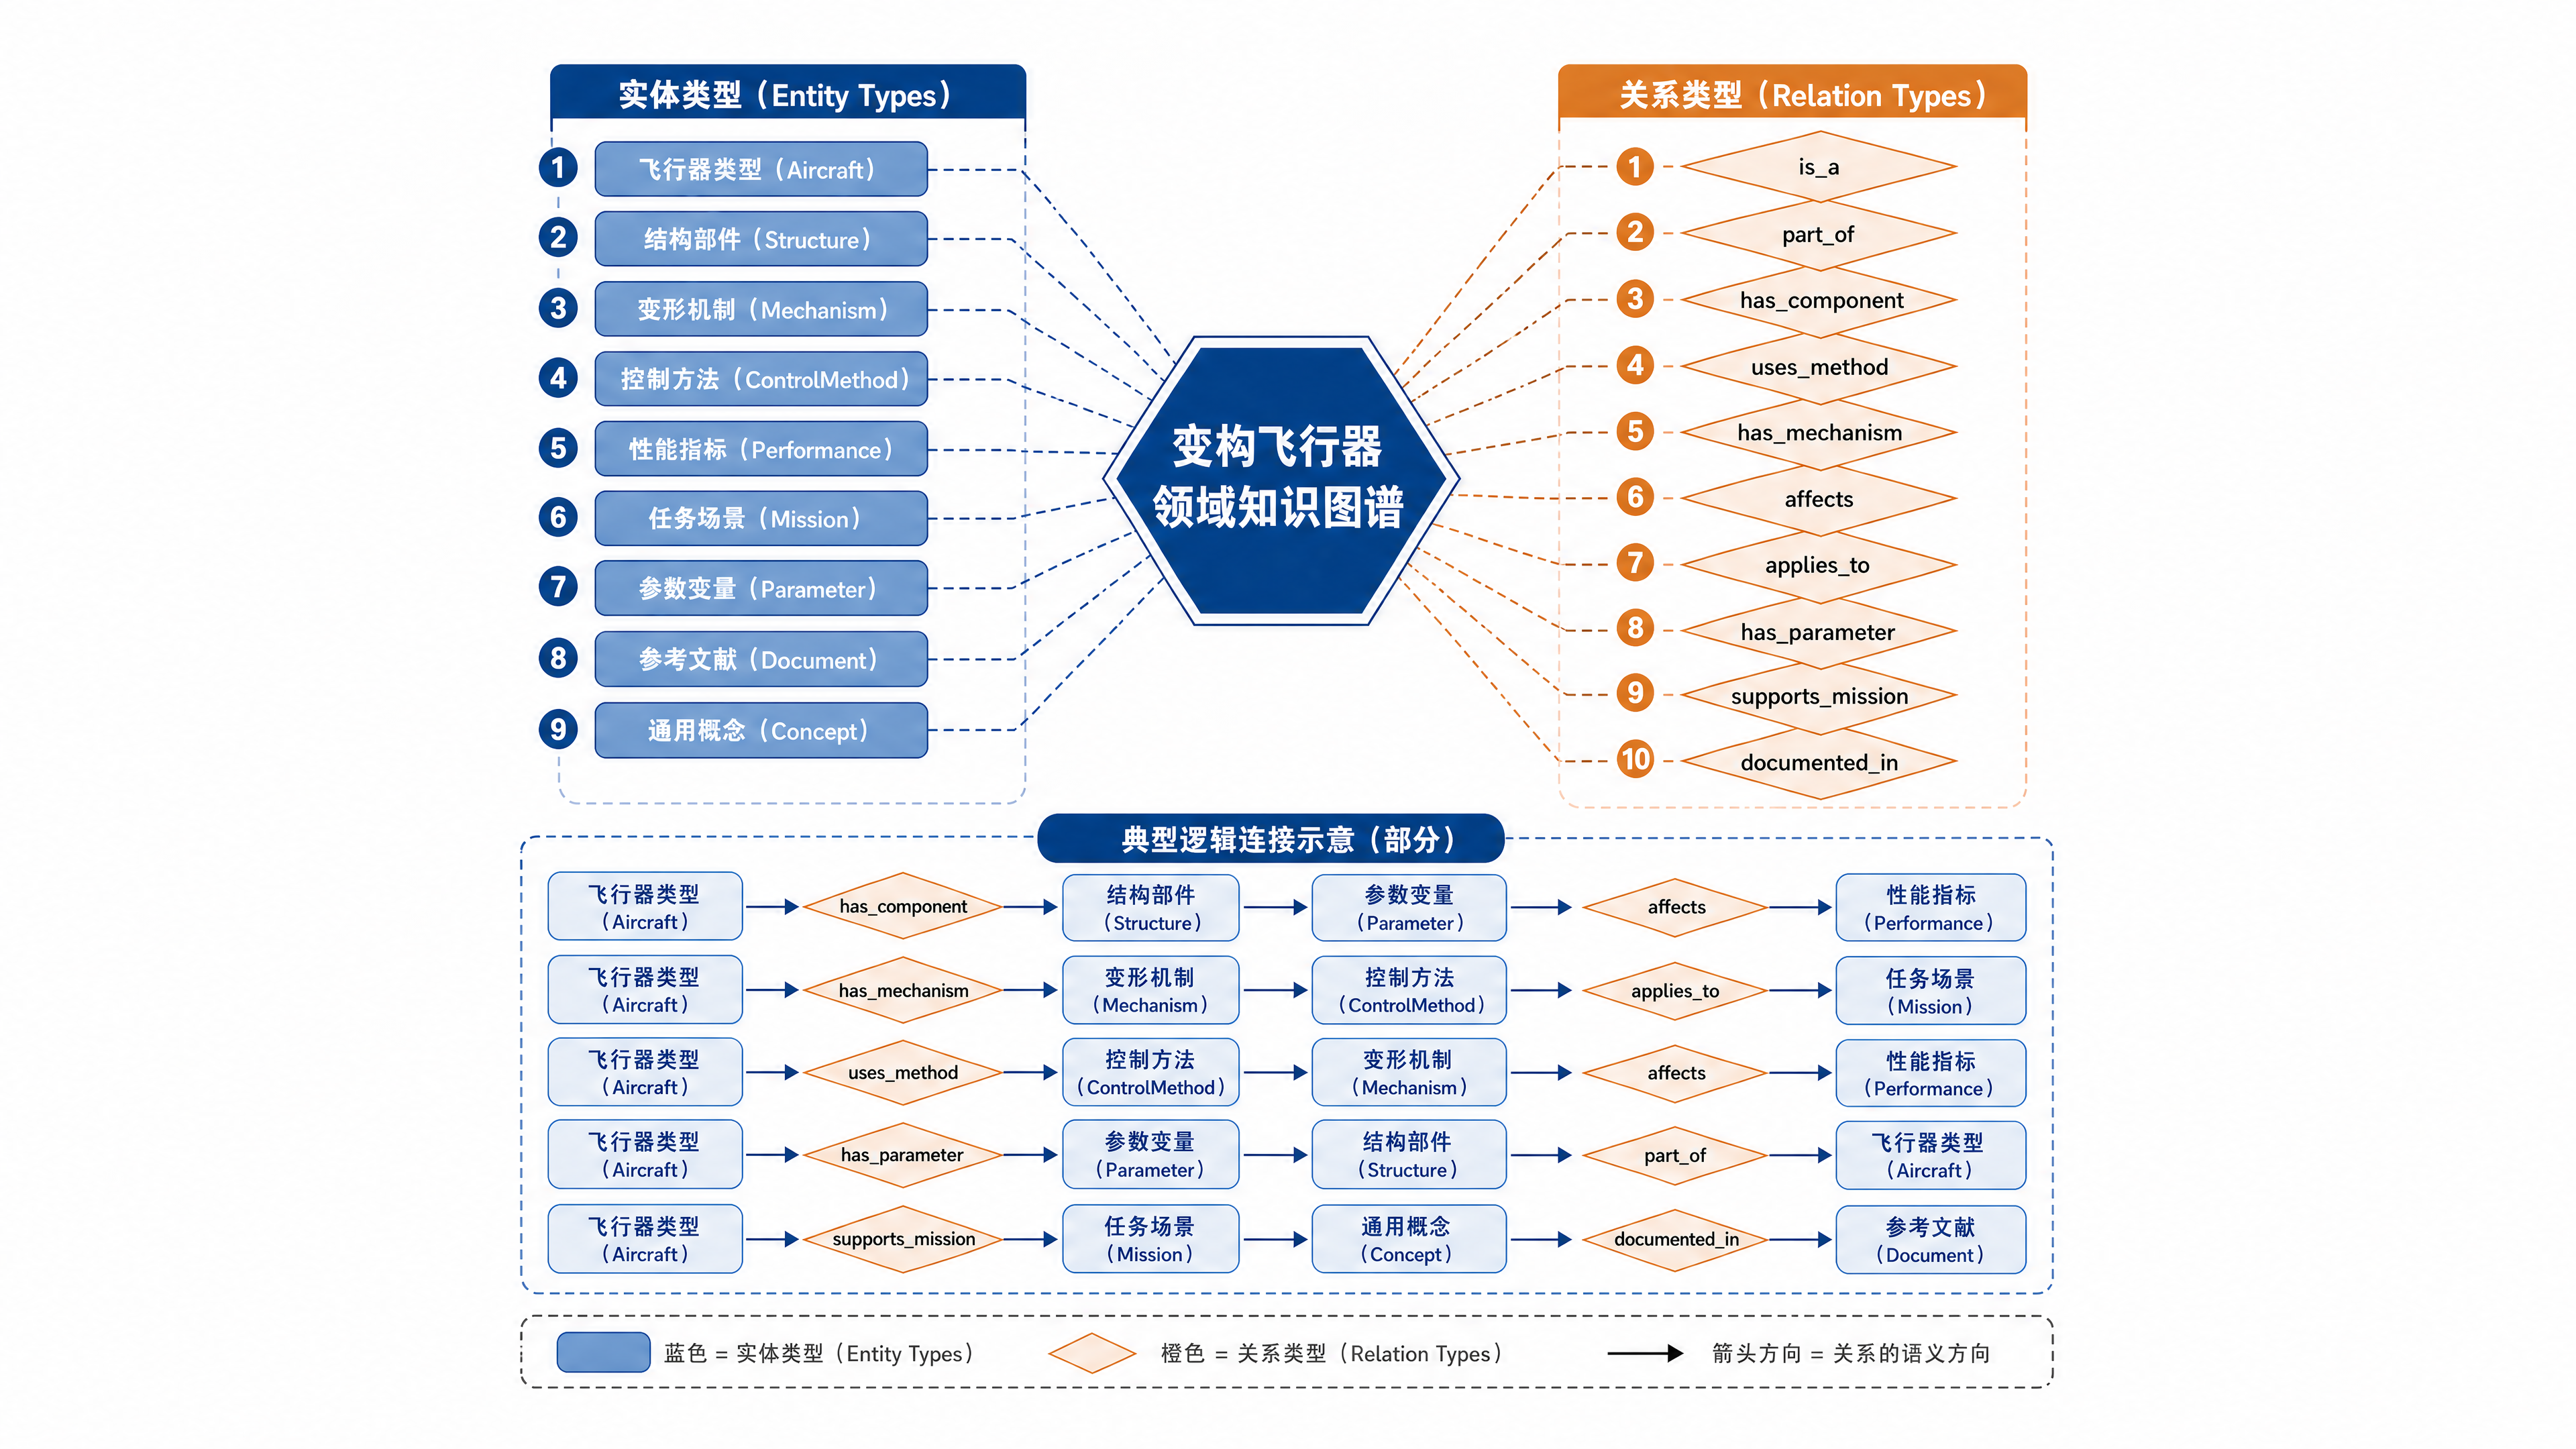
\includegraphics[width=0.85\textwidth]{figures/实体类型与关系类型本体结构图.png}
\caption{实体类型与关系类型本体结构图}
\end{figure}

\begin{figure}[H]\centering
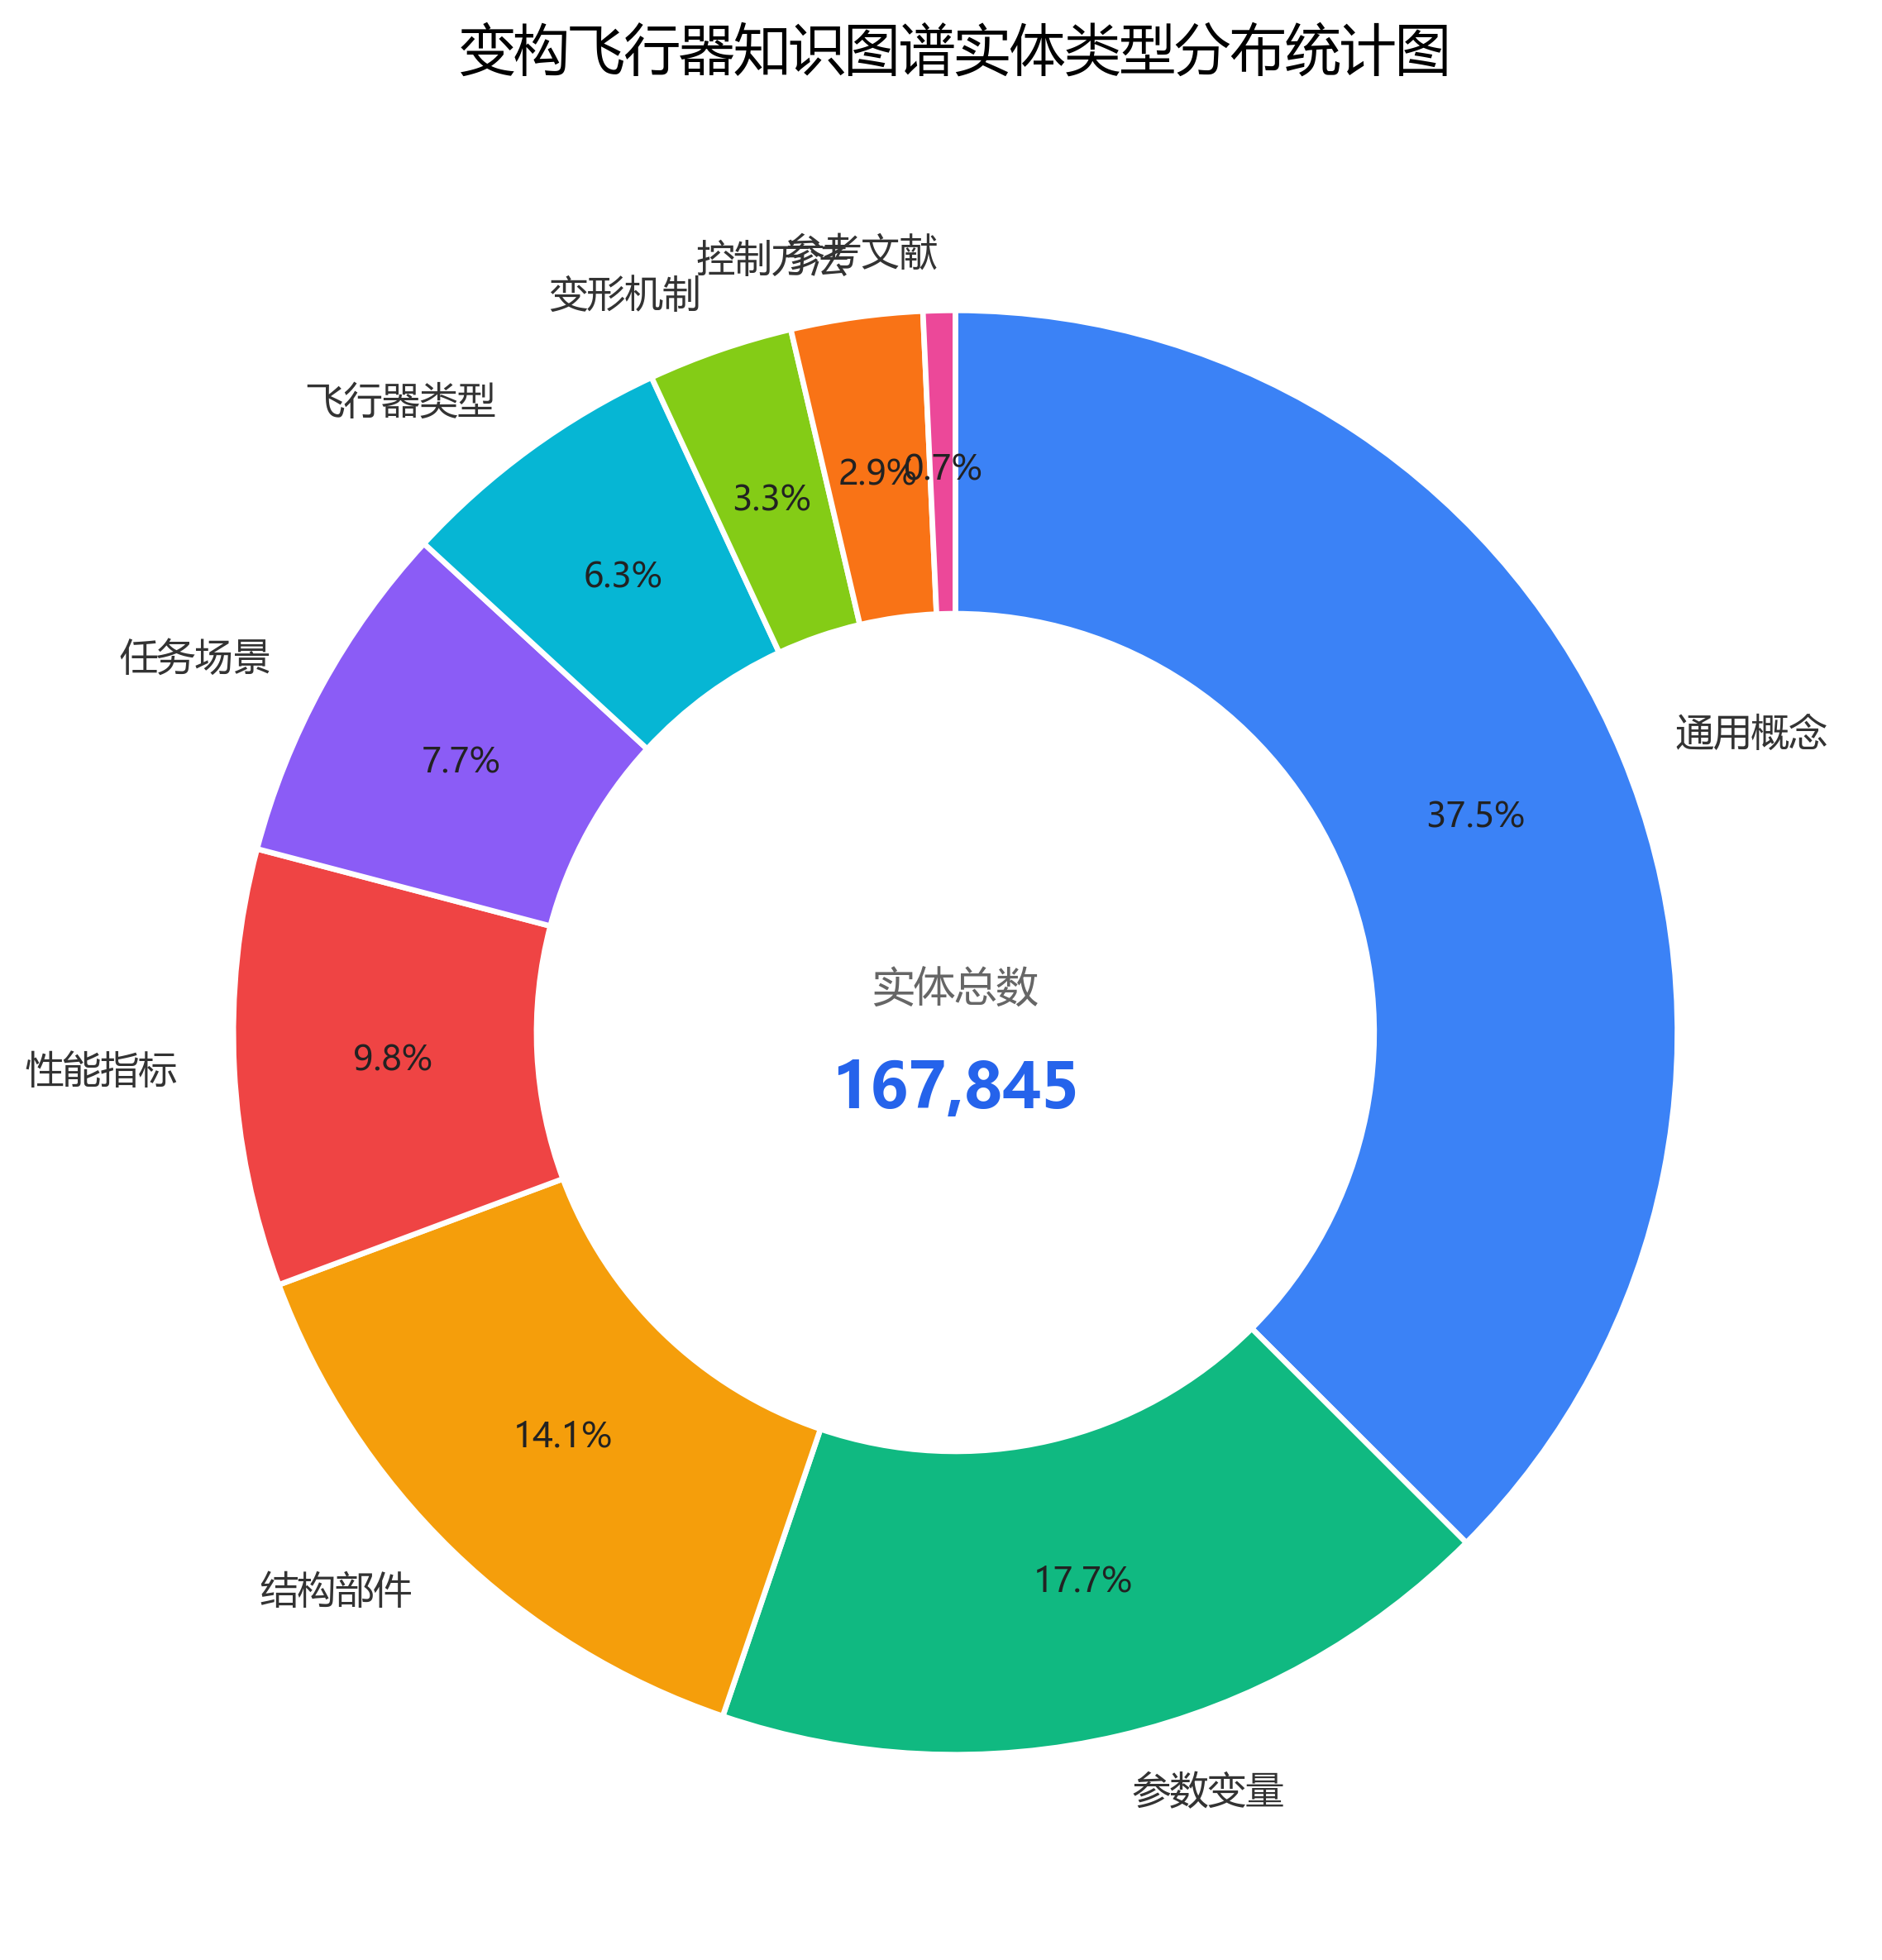
\includegraphics[width=0.5\textwidth]{figures/实体类型分布统计图.png}
\caption{实体类型分布统计图}
\end{figure}

从统计结果看，\texttt{Concept}、\texttt{Parameter} 和 \texttt{Structure} 类型占比最高，说明图谱同时覆盖了大量通用概念、参数知识和结构知识。这与变构飞行器领域“概念体系复杂、结构设计突出、参数分析频繁”的学科特点一致。实体类型体系不仅服务于分类统计，也为后续关系抽取约束提供语义边界。

\subsection{关系类型设计与语义约束}
项目共设计 10 类关系，其中最终结果中主要出现 \texttt{is\_a}、\texttt{has\_component}、\texttt{part\_of}、\texttt{affects}、\texttt{uses\_method}、\texttt{has\_mechanism}、\texttt{supports\_mission}、\texttt{applies\_to} 和 \texttt{has\_parameter}。这些关系覆盖概念层级、结构组成、方法使用、参数影响和任务适用等多种逻辑模式。

\begin{figure}[H]\centering
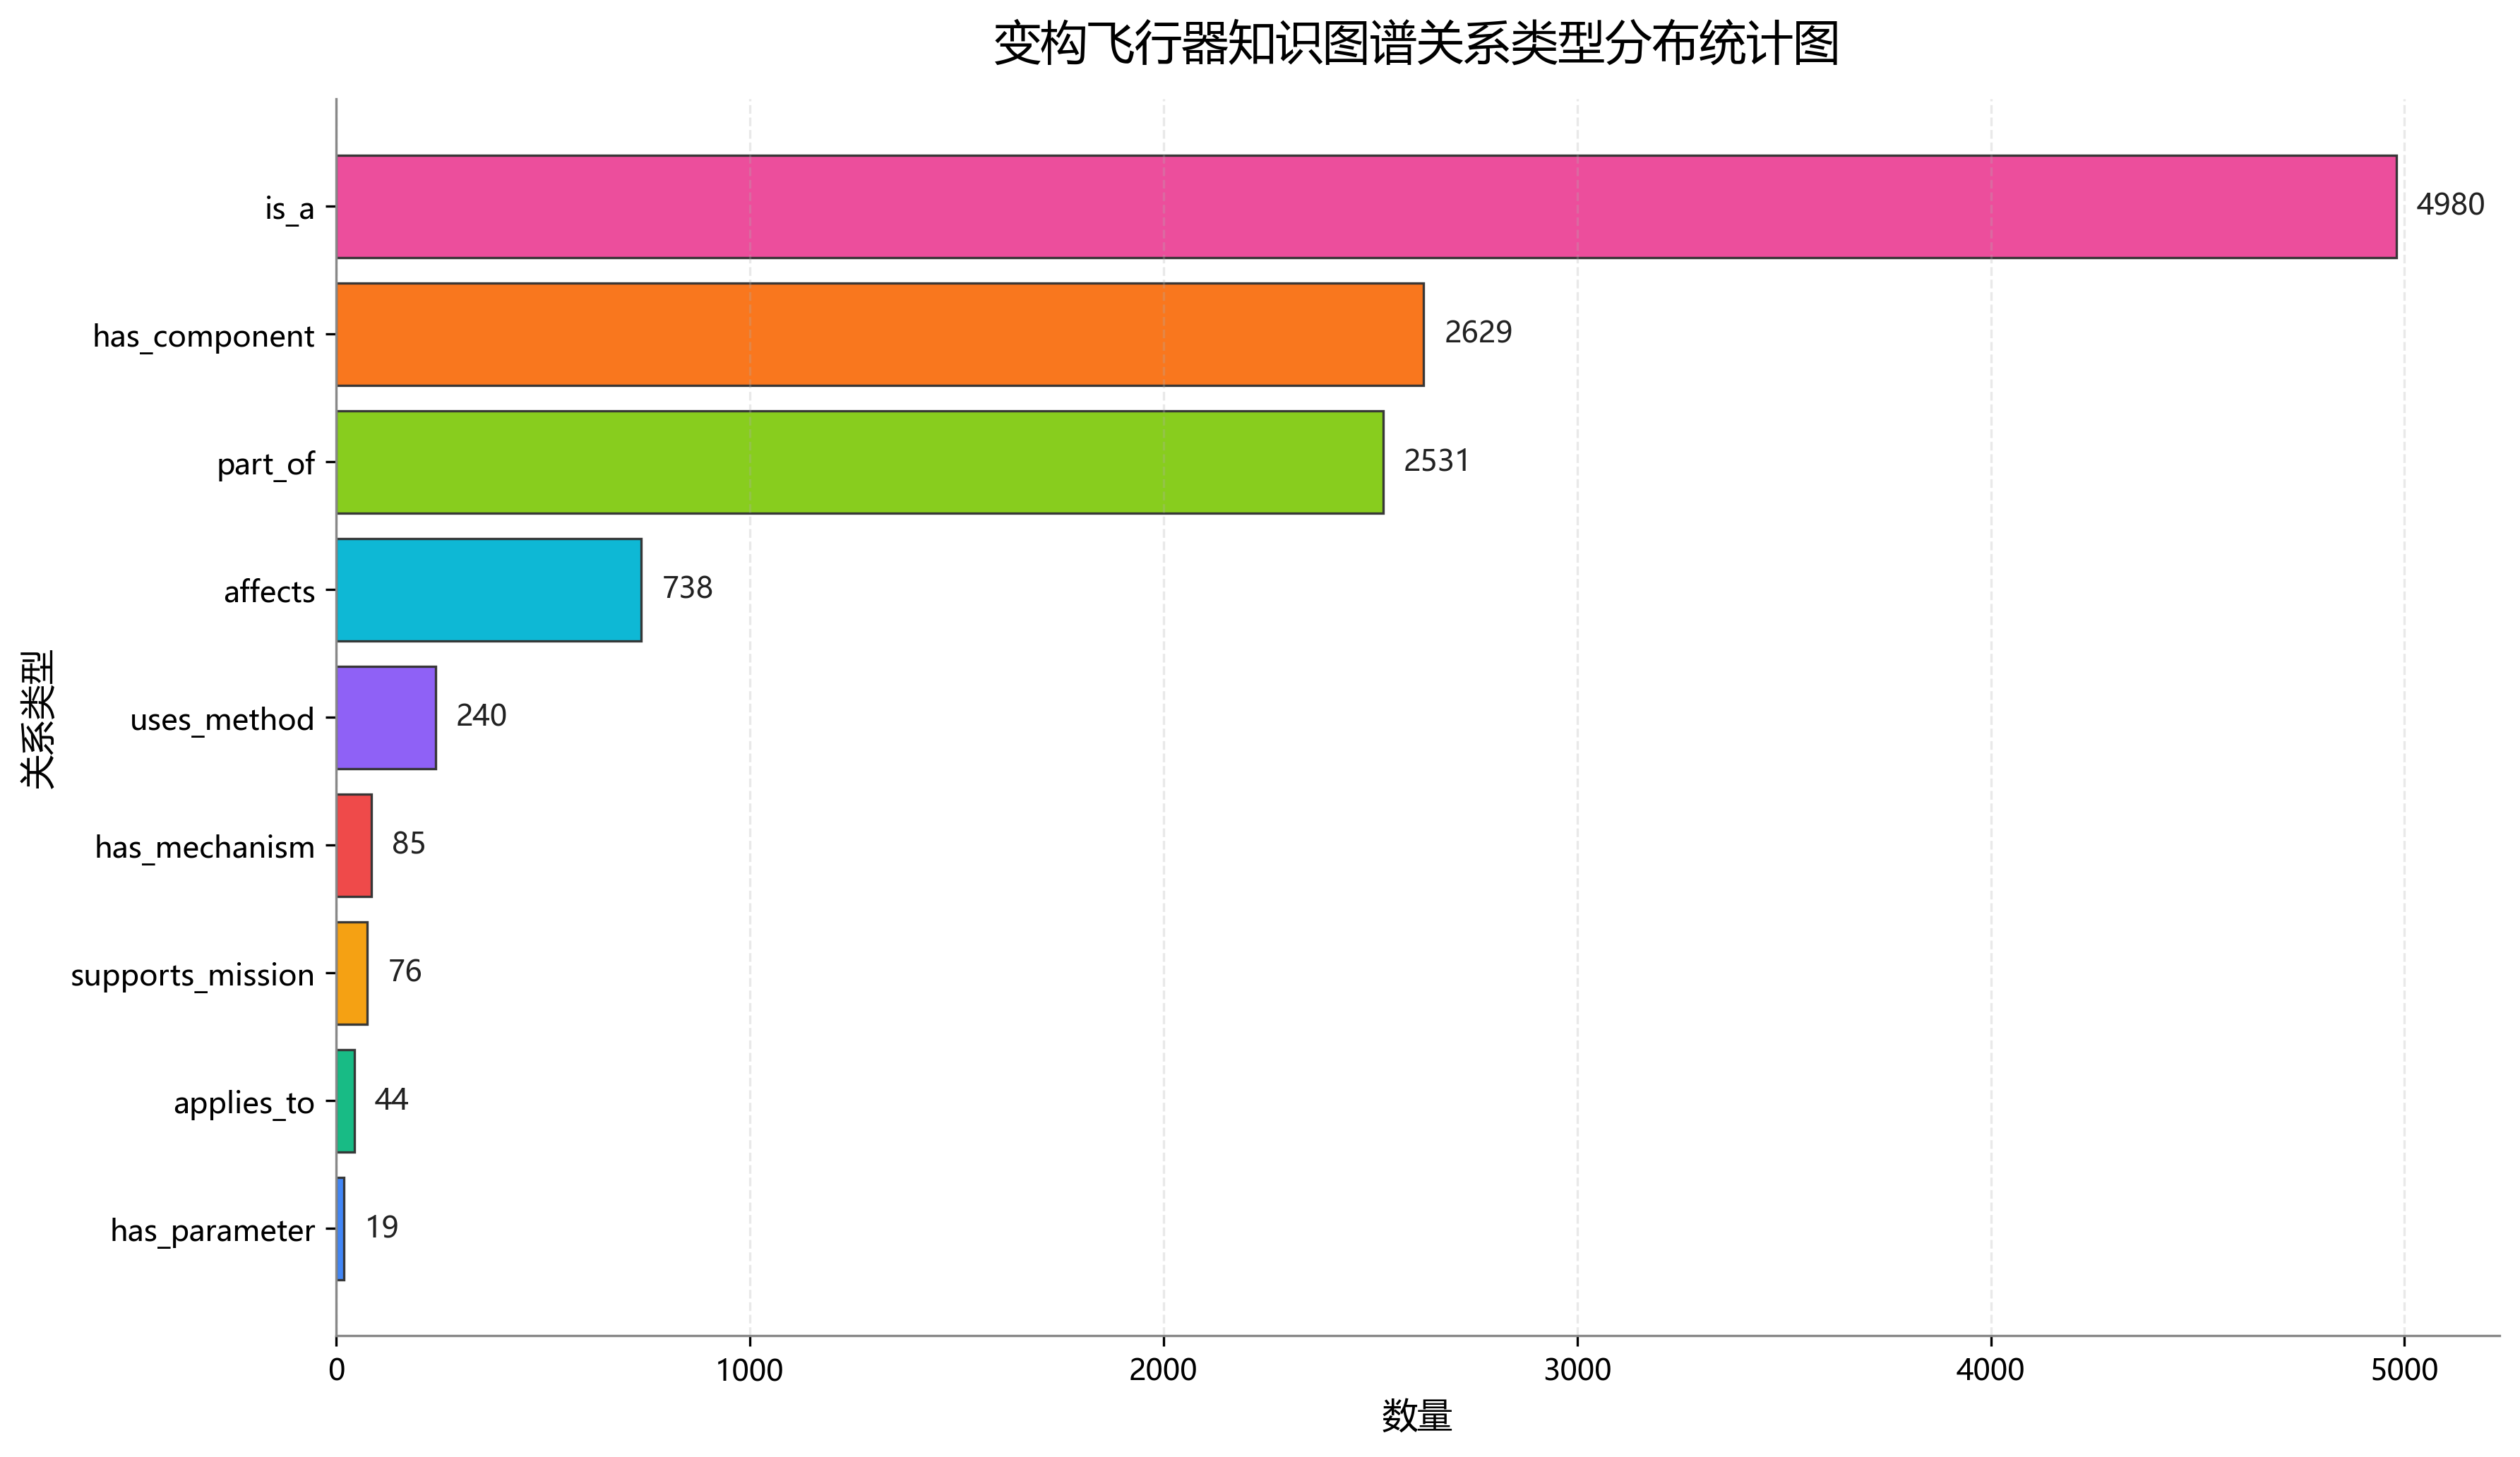
\includegraphics[width=0.82\textwidth]{figures/关系类型分布统计图.png}
\caption{关系类型分布统计图}
\end{figure}

统计结果表明，\texttt{is\_a}、\texttt{has\_component} 和 \texttt{part\_of} 是图谱中占比最高的三类关系，这说明当前图谱在概念层次和组成关系方面最为密集。若记关系为 \(r\)，头尾实体类型分别为 \(h_t\) 与 \(t_t\)，则合法关系可抽象表示为
\[
\mathcal{I}(r,h_t,t_t)=1 \iff (h_t,t_t)\in \Omega_r
\]
其中 \(\Omega_r\) 为关系 \(r\) 的允许类型组合集合。通过这种类型约束，系统有效降低了不合理三元组数量。

\subsection{术语归一化与别名映射机制}
由于领域文献中存在中文全称、英文缩写、修饰性短语等多种表达，项目在术语定稿阶段构建了规范名称与别名映射机制。设原始表达为 \(a\)，规范概念为 \(c\)，则归一化过程可表示为 \(\phi(a)=c\)。这一机制可显著减少图谱中的重复节点，提高搜索和关系聚合效果，也是前端展示稳定性的关键基础。
